\chapter{Projectresultaat}

Het project zal worden uitgevoerd om, als projectgroep, ervaring op te doen met
embedded vision. Het uiteindelijke doel van het project is om de Nerf-gun
(gebouwd tijdens vorig project, figuur \ref{fig:nerf}) volledig zelfstandig en
zo snel mogelijk te laten draaien. De Nerf-gun schiet op een object met als
kenmerk een gekleurd rondje.

Het project zal uiterlijk in week 20 van het schooljaar functioneel moeten
zijn. De opdracht kan dus worden geformuleerd als:

\begin{quotation}
\emph{Uiterlijk week 20 van het academisch jaar 2013-2014 zal een systeem
ontwikkeld zijn die autonoom een Nerf-gun kan afvuren op bewegende, gemarkeerde,
doelwitten. Het systeem moet gebruik maken van camera beelden om deze doelwitten
te vinden binnen een omgeving.}
\end{quotation}

Het is de bedoeling dat het systeem volledig onafhankelijk kan functioneren.
Dit betekend dat de logica draait op een embedded systeem. Verdere opties voor
het systeem zijn:

\begin{itemize}
    \item De kleur van een rondje een haatfactor meegeven. Dit betekend dat er
        meer pijltjes bij een bepaalde kleur worden afgeschoten;
    \item het camera beeld weergeven op een display;
    \item of de Nerf-gun direct bedienen via een touch screen display of via
        knoppen.
\end{itemize}

\begin{figure}
	\begin{center}
		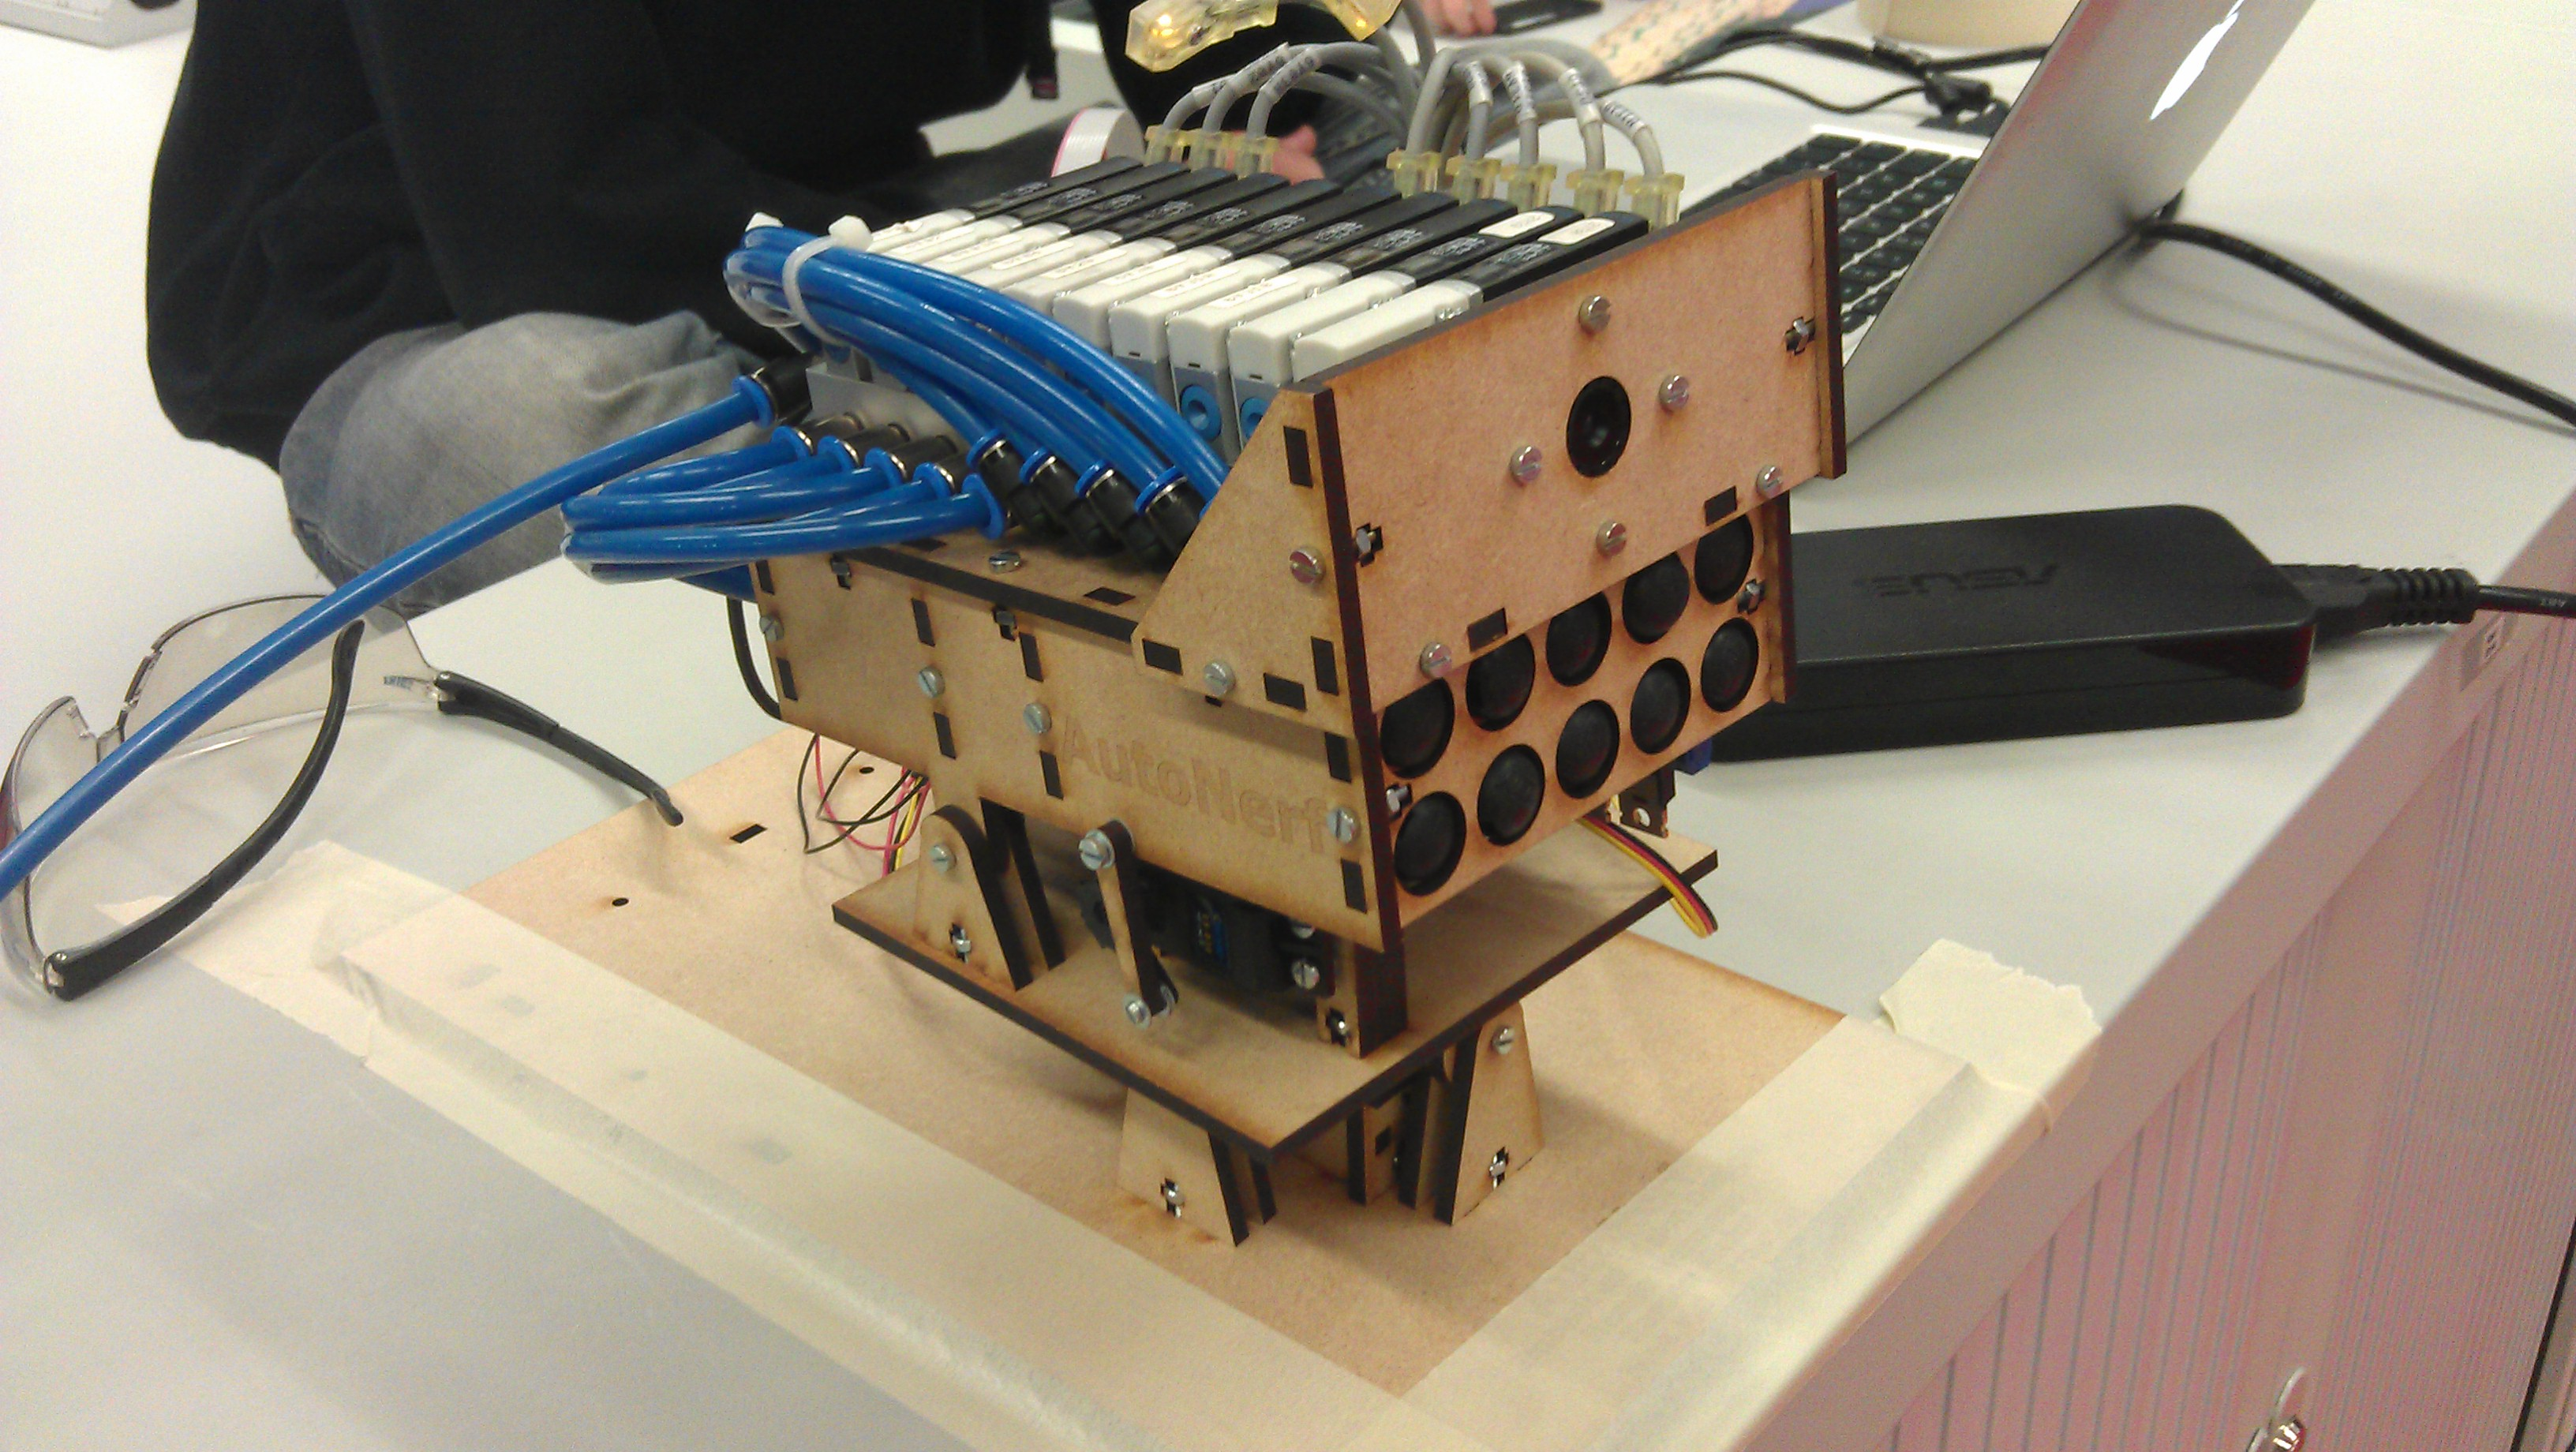
\includegraphics[scale=0.1]{figures/autonerf.jpg}
	\end{center}
    \caption{Het zelf-ontwikkelde Nerf-gun systeem}
    \label{fig:nerf}
\end{figure}
